\documentclass[12pt, a4paper]{report}

% Packages :

\usepackage[french]{babel}
\usepackage[utf8]{inputenc}
\usepackage[T1]{fontenc}
\usepackage[pdftex, pdfauthor={Bacomathiques}]{hyperref}
\usepackage{sectsty}
\usepackage[explicit]{titlesec}
\usepackage{xcolor}
\usepackage{amsmath}
\usepackage{amssymb}
\usepackage{amsthm}
\usepackage{fourier}
\usepackage{titlesec}
\usepackage{fancyhdr}
\usepackage{catchfilebetweentags}
\usepackage[french, capitalise, noabbrev]{cleveref}
\usepackage[fit, breakall]{truncate}
\usepackage[margin=3cm]{geometry}
\usepackage{tocloft}
\usepackage{tikz}
\usepackage{tocloft}
\usepackage{microtype}
\usepackage{listings}
\usepackage{tabularx}
\usepackage{calc}
\usepackage[export]{adjustbox}
\usepackage[most]{tcolorbox}
\usepackage{standalone}
\usepackage{xlop}
\usepackage{etoolbox}
\usepackage{environ}

\usetikzlibrary{arrows.meta}
\usetikzlibrary{trees}

% Paramètres :

\author{Bacomathiques}
\definecolor{graphe}{HTML}{93c9ff}
\setcounter{MaxMatrixCols}{12}
\setlength{\parindent}{0pt}
\setlength{\fboxsep}{0pt}
%\pdfsuppresswarningpagegroup=1

% Code :

\lstdefinestyle{style}{
	backgroundcolor=\color{white},
	commentstyle=\em\color[HTML]{999988},
	keywordstyle=\bfseries,
	identifierstyle=\normalfont,
	stringstyle=\color[rgb]{0.87, 0.07, 0.27},
	basicstyle=\ttfamily\color{black},
	breakatwhitespace=false,
	breaklines=true,
	captionpos=b,
	keepspaces=true,
	numbers=left,
	numbersep=5pt,
	showspaces=false,
	showstringspaces=false,
	showtabs=false,
	tabsize=2,
	numbers=none
}

\lstset{style=style}
\lstset{
	literate=
	{á}{{\'a}}1
	{à}{{\`a}}1
	{ã}{{\~a}}1
	{é}{{\'e}}1
	{ê}{{\^e}}1
	{í}{{\'i}}1
	{ó}{{\'o}}1
	{õ}{{\~o}}1
	{ú}{{\'u}}1
	{ü}{{\"u}}1
	{ç}{{\c{c}}}1
}

\lstset{
	framextopmargin=10pt,
	framexrightmargin=10pt,
	framexbottommargin=10pt,
	framexleftmargin=10pt,
	xleftmargin=10pt,
	xrightmargin=10pt,
}

% Couleurs :

\definecolor{title}{HTML}{912c21}
\definecolor{section}{HTML}{1c567d}
\definecolor{subsection}{HTML}{2980b9}

\definecolor{rule}{HTML}{c4c4c4}

\definecolor{formula}{HTML}{ebf3fb}
\definecolor{formula-left}{HTML}{3583d6}

\definecolor{tip}{HTML}{dcf3d8}
\definecolor{tip-left}{HTML}{26a65b}

\definecolor{demonstration}{HTML}{fff8de}
\definecolor{demonstration-left}{HTML}{f1c40f}

\definecolor{exercise}{HTML}{e0f2f1}
\definecolor{exercise-left}{HTML}{009688}

\definecolor{correction}{HTML}{e0f7fa}
\definecolor{correction-left}{HTML}{00bcd4}

\definecolor{toc}{HTML}{fceae9}
\definecolor{toc-left}{HTML}{e74c3c}
\definecolor{toc-dark}{HTML}{87281f}

% Titres :

\renewcommand{\thesection}{\Roman{section} - }
\renewcommand{\thesubsection}{\arabic{subsection}. }

\newcommand{\sectionstyle}{\normalfont\LARGE\bfseries\color{section}}
\titleformat{\section}{\sectionstyle}{\thesection #1}{0pt}{}
\titleformat{name=\section, numberless}{\sectionstyle}{#1}{0pt}{}

\newcommand{\subsectionstyle}{\normalfont\Large\bfseries\color{subsection}}
\titleformat{\subsection}{\subsectionstyle}{\thesubsection #1}{0pt}{}
\titleformat{name=\subsection, numberless}{\subsectionstyle}{#1}{0pt}{}

\titlelabel{\thetitle\ }

% Table des matières :

\addto\captionsfrench{\renewcommand\contentsname{}}
\renewcommand{\cftsecpagefont}{\color{toc-dark}}
\renewcommand{\cftsubsecpagefont}{\color{toc-dark}}
\renewcommand{\cftsecleader}{\cftdotfill{\cftdotsep}}
\renewcommand{\cftsecfont}{\bfseries}
\renewcommand{\cftsecpagefont}{\bfseries\color{toc-dark}}
\setlength{\cftbeforetoctitleskip}{0pt}
\setlength{\cftaftertoctitleskip}{0pt}
\setlength{\cftsecindent}{0pt}
\setlength{\cftsubsecindent}{20pt}
\setlength{\cftsubsecnumwidth}{20pt}

% Commandes :

\newcommand{\newpar}{\\[\medskipamount]}
\newcommand{\lesson}[3]{%
	\newcommand{\level}{#1}%
	\newcommand{\id}{#2}%
	\hypersetup{pdftitle={#3}}
	\begin{center}%
		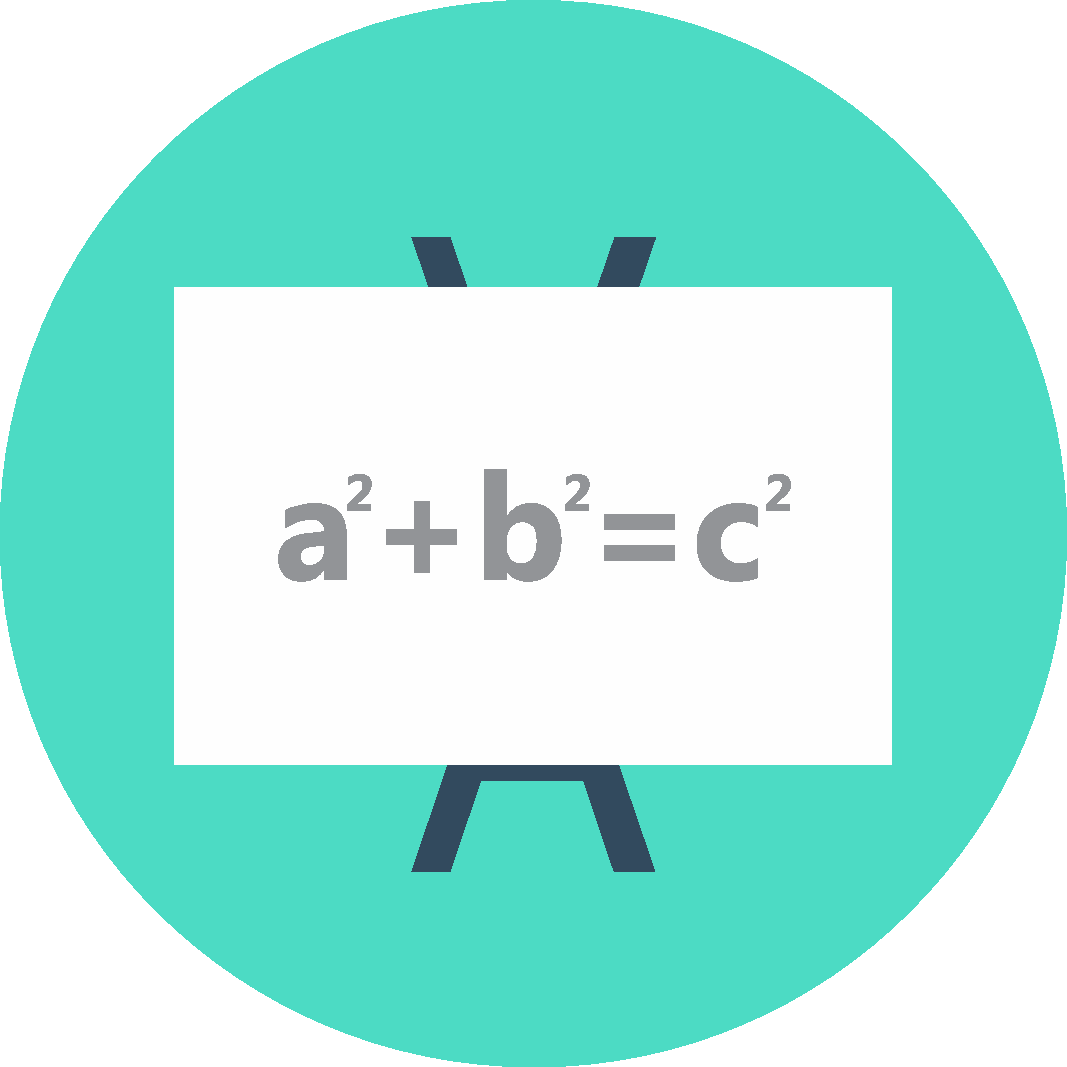
\includegraphics[width=150px]{\imagespath/bacomathiques}%
		
		\vspace{30pt}%
		{\Huge\color{title} #3}%
		
		\vspace{10pt}%
		{Bacomathiques --- \href{https://bacomathiqu.es/cours/#1/#2}{\color{section} https://bacomathiqu.es}}%
		
		\vspace{20pt}%
	\end{center}%
	\begin{toc}
		\tableofcontents%
	\end{toc}
	\thispagestyle{empty}%
	\newpage%
	\setcounter{page}{1}%
}
\newcommand{\imagespath}{../../images}
\newcommand{\lessonimagespath}{\imagespath/lessons/\level/\id/}
\newcommand{\includelatexpicture}[2][\textwidth - 100pt]{%
	\begin{center}%
		\resizebox{#1}{!}{%
			\input{\lessonimagespath#2}%
		}%
	\end{center}%
	\medskip%
}
\newcommand{\includeimage}[1]{%
	\begin{center}%
		\includegraphics{\lessonimagespath#1}%
	\end{center}%
	\medskip%
}
\newcommand{\includerepresentation}[1]{%
	\begin{center}%
		\setlength{\fboxrule}{0.5pt}%
		\href{https://www.geogebra.org/m/#1}{\includegraphics[width=\textwidth-1pt,fbox]{\lessonimagespath#1}}%
	\end{center}%
}
\newcommand{\floor}[1]{\lfloor #1 \rfloor}

\makeatletter
\newcommand\inputcontent{\@ifstar{\inputcontent@star}{\inputcontent@nostar}}
\newcommand{\inputcontent@star}[1]{%
	\ExecuteMetaData[#1]{content}%
}
\newcommand{\inputcontent@nostar}[1]{%
	\newpage%
	\inputcontent@star{#1}%
}
\makeatother

\let\oldsection\section
\renewcommand\section{\clearpage\oldsection}
\newcommand{\contentwidth}[1][medium]{}

% En-têtes :

\pagestyle{fancy}

\renewcommand{\sectionmark}[1]{\markboth{\thesection \ #1}{}}

\fancyhead[R]{\truncate{0.23\textwidth}{\color{title}\thepage}}
\fancyhead[L]{\truncate{0.73\textwidth}{\color{title}\leftmark}}
\fancyfoot[C]{\scriptsize \href{https://bacomathiqu.es/cours/\level/\id}{\texttt{bacomathiqu.es}}}

\makeatletter
\patchcmd{\f@nch@head}{\rlap}{\color{rule}\rlap}{}{}
\patchcmd{\headrule}{\hrule}{\color{rule}\hrule}{}{}
\makeatother

% Environnements :

\newenvironment{nosummary}{}{}
\newcommand{\tcolorboxtitle}[2]{\setlength{\fboxsep}{2.5pt}\hspace{-10pt}\colorbox{#1-left}{\hspace{8pt}\MakeUppercase{#2} \hspace{2pt} \includegraphics[height=0.8em]{\imagespath/bubbles/#1}\hspace{5pt}}}
\newcommand{\tcolorboxsubtitle}[2]{\ifstrempty{#2}{}{\textcolor{#1-left}{\large#2}\\[\medskipamount]}}
\tcbset{
	frame hidden,
	boxrule=0pt,
	boxsep=0pt,
	enlarge bottom by=8.5pt,
	enhanced jigsaw,
	boxed title style={sharp corners,boxrule=0pt,coltitle={white},titlerule=0pt},
	fonttitle=\fontsize{6pt}{6pt}\bfseries\boldmath,
	top=10pt,
	right=10pt,
	bottom=10pt,
	left=10pt,
	arc=0pt,
	outer arc=0pt,
}
\newtcolorbox{toc}[1][]{
	colback=toc,
	borderline west={3pt}{0pt}{toc-left},
	title=\tcolorboxtitle{toc}{Table des matières},
	colbacktitle=toc,
	before upper={\tcolorboxsubtitle{toc}{#1}}
}
\newtcolorbox{formula}[1][]{
	colback=formula,
	borderline west={3pt}{0pt}{formula-left},
	title=\tcolorboxtitle{formula}{À retenir},
	colbacktitle=formula,
	before upper={\tcolorboxsubtitle{formula}{#1}}
}
\newtcolorbox{tip}[1][]{
	colback=tip,
	borderline west={3pt}{0pt}{tip-left},
	title=\tcolorboxtitle{tip}{À lire},
	colbacktitle=tip,
	before upper={\tcolorboxsubtitle{tip}{#1}}
}
\newtcolorbox{demonstration}[1][]{
	colback=demonstration,
	borderline west={3pt}{0pt}{demonstration-left},
	title=\tcolorboxtitle{demonstration}{Démonstration},
	colbacktitle=demonstration,
	before upper={\tcolorboxsubtitle{demonstration}{#1}}
}

\NewEnviron{whitetabularx}[1]{%
	\renewcommand{\arraystretch}{2.5}
	\colorbox{white}{%
		\begin{tabularx}{\textwidth}{#1}%
			\BODY%
		\end{tabularx}%
	}%
}

% Longueurs :

\newlength{\espacetitreliste}
\setlength{\espacetitreliste}{-16pt}
\newcommand{\entretitreetliste}{\vspace{\espacetitreliste}}

\begin{document}
	%<*content>
	\lesson{terminale}{10}{lois-bernoulli-binomiale}{Lois de Bernoulli et binomiale}

	\header{caption}{Ces lois jouent un rôle dans l'étude des décisions binaires.}

	\header{description}{La loi binomiale (qui est en quelque sorte, une généralisation de la loi
		de Bernoulli) aide à la modélisation de décisions binaires. Ce chapitre va tout
		d'abord effectuer quelques rappels sur les variables aléatoires, puis va donner
		des propriétés que possèdent les loi de Bernoulli et binomiale (espérance, variance,
		écart-type, etc...).}

	\header{difficulty}{4}

	\section{Rappels sur les variables aléatoires}

	\subsection{Définition}

	Nous allons rappeler quelques notions vues en classe de Première sur les variables aléatoires.

	\begin{formula}[Définition]
		Une \textbf{variable aléatoire} $X$ est une fonction qui, à chaque événement élémentaire de l'univers $\Omega$ y associe un nombre réel. C'est-à-dire : $X : \Omega \rightarrow \mathbb{R}$.
	\end{formula}

	\subsection{Loi de probabilité}

	\begin{formula}[Définition]
		Soit $X$ une variable aléatoire. La \textbf{loi de probabilité} de $X$ attribue à chaque valeur $x_i$ la probabilité $p_i = P(X = x_i)$ de l'événement $X = x_i$ constitué de tous les événements élémentaires dont l'image par $X$ est $x_i$.
	\end{formula}

	On représente généralement les lois de probabilité par un tableau.

	\begin{formula}[Représentation d'une loi de probabilité par un tableau]
		Soit $X$ une variable aléatoire. On peut représenter sa loi de probabilité par le tableau ci-contre :
		\newpar
		\begin{whitetabularx}{|X|X|X|X|X|}
			\hline
			$x_i$ & $x_1$ & $x_2$ & ... & $x_n$ \\
			\hline
			$p_i$ \newline $=P(X = x_i)$ & $p_1$ \newline $= P(X = x_1)$ & $p_2$ \newline $= P(X = x_2)$ & ... & $p_n$ \newline $= P(X = x_n)$ \\
			\hline
		\end{whitetabularx}
		\newpar
		On a $p_1 + p_2 + \dots + p_n = 1$.
	\end{formula}

	\begin{tip}
		Cette définition peut sembler un peu compliquée mais elle signifie juste qu'une loi de probabilité assigne une probabilité à chaque valeur prise par notre variable aléatoire.
	\end{tip}

	\subsection{Espérance, variance et écart-type}

	\begin{formula}[Espérance]
		L'\textbf{espérance} $E(X)$ d'une variable aléatoire $X$ est le réel :
		\[ E(X) = x_1 \times p_1 + x_2 \times p_2 + \dots + x_n \times p_n \]
	\end{formula}

	\begin{formula}[Variance et écart-type]
		La \textbf{variance} $V(X)$ et l'\textbf{écart-type} $\sigma(X)$ d'une variable aléatoire $X$ sont les réels positifs suivants :
		\begin{itemize}
			\item $V(X) = E(X^2) - E(X)^2$
			\item $\sigma(X) = \sqrt{V(X)}$
		\end{itemize}
	\end{formula}

	\begin{tip}[Exemple]
		Calcul de l'espérance, de la variance et de l'écart-type. Soit $X$ une variable aléatoire suivant la loi de probabilité donnée par le tableau ci-dessous :
		\newpar
		\begin{whitetabularx}{|X|X|X|X|X|}
			\hline
			$x_i$ & $-1$ & $0$ & $2$ & $6$ \\
			\hline
			$p_i$ & $\frac{1}{4}$ & $\frac{1}{2}$ & $\frac{1}{8}$ & $\frac{1}{8}$ \\
			\hline
		\end{whitetabularx}
		\newpar
		On a :
		\begin{itemize}
			\item $E(X) = -1 \times \frac{1}{4} + 0 \times \frac{1}{2} + 2 \times \frac{1}{8} + 6 \times \frac{1}{8} = \frac{3}{4}$
			\item $V(X) = ((-1)^2 \times \frac{1}{4} + 0^2 \times \frac{1}{2} + 2^2 \times \frac{1}{8} + 6^2 \times \frac{1}{8}) - (\frac{3}{4})^2 = \frac{75}{16}$
			\item $\sigma(X) = \sqrt{\frac{75}{16}} \approx 2.165$
		\end{itemize}
	\end{tip}

	Chacun de ces paramètres a une utilité bien précise. En effet :

	\begin{formula}[Signification des paramètres]
		\entretitreetliste
		\begin{itemize}
			\item L'espérance est la \textbf{valeur moyenne} prise par $X$.
			\item La variance et l'écart-type mesurent la \textbf{dispersion} des valeurs prises par $X$. Plus ces valeurs sont grandes, plus les valeurs sont dispersées autour de l'espérance.
		\end{itemize}
	\end{formula}

	\section{Loi de Bernoulli}

	\subsection{Succession d'épreuves indépendantes}

	\begin{formula}[Univers associé]
		Soit une succession de $n$ épreuves indépendantes (c'est-à-dire que le résultat de l'une n'a pas d'incidence sur le résultat de la suivante). On note les univers associés à chaque expérience respectivement par $\Omega_1$, $\Omega_2$, ... , $\Omega_n$.
		\newpar
		Alors l'univers associé à cette succession d'épreuves indépendantes est le produit cartésien $\Omega_1 \times \Omega_2 \times \dots \times \Omega_n$.
	\end{formula}

	\begin{tip}[Exemple]
		On effectue deux lancers de dé équilibrés à $6$ faces. Ces lancers sont indépendants et admettent $\Omega_1 = \{1; \dots; 6\} = \Omega_2$ pour univers.
		\newpar
		Ainsi, l'univers associé à cette succession de $2$ épreuves indépendantes est $\Omega_1 \times \Omega_2 = \{1; \dots; 6\} \times \{1; \dots; 6\}$.
		\newpar
		Par exemple, une issue possible à cette succession d'épreuves est $(1; 6)$ (qui correspond au fait de faire un $1$ avec le premier dé et de faire un $6$ avec le deuxième dé).
	\end{tip}

	\begin{tip}[Arbre de probabilité]
		Il est tout à fait possible de modéliser ce type d'expérience à l'aide d'un arbre de probabilité. Cependant, cela peut devenir compliqué dès lors que le nombre d'épreuves dépasse $2$ ou que le nombre d'issues possibles dépasse $3$.
		\newpar
		Un arbre de probabilité permet également de représenter une succession d'épreuves non-indépendantes.
	\end{tip}

	\begin{formula}[Calcul de probabilité]
		Soit une succession de $n$ épreuves indépendantes et soit $(\omega_1, \dots, \omega_n)$ une issue de cette succession d'épreuves. Alors $P((\omega_1, \dots, \omega_n)) = P(\omega_1) \times \dots \times P(\omega_n)$.
	\end{formula}

	\begin{tip}[Exemple]
		En reprenant les notations de l'exemple précédent, on a $P((1; 6)) = P(1) \times P(6) = \frac{1}{36}$.
		\newpar
		D'ailleurs, on se trouve dans une situation \textbf{d'équiprobabilité} car toutes les issues ont une probabilité de $\frac{1}{36}$ de se produire.
	\end{tip}

	\subsection{Épreuve et schéma de Bernoulli}

	Derrière ces noms qui peuvent sembler compliquer, se cache une notion finalement simple, et que l'on rencontre souvent dans la vie quotidienne.

	\begin{formula}[Épreuve de Bernoulli]
		Une \textbf{épreuve de Bernoulli} est une expérience aléatoire qui n'admet que deux issues possibles : le succès et l'échec.
	\end{formula}

	\begin{tip}
		Tout choix aléatoire binaire est une épreuve de Bernoulli. On peut donner l'exemple d'un lancer de pièce, obtenir un résultat durant un lancer de dé, ou même le fait que vous décidiez de laisser une bonne note ou non à l'application ``Bacomathiques'' !
	\end{tip}

	Il est souvent possible de répéter plusieurs fois une épreuve de Bernoulli. C'est ce qu'on appelle un \textbf{schéma de Bernoulli}.

	\begin{formula}[Schéma de Bernoulli]
		Soit une succession d'épreuves de Bernoulli indépendantes. On appelle cette succession un schéma de Bernoulli.
	\end{formula}

	\subsection{Loi de Bernoulli}

	\begin{formula}[Définition]
		Soient $X$ une variable aléatoire et $p \in ]0; 1[$. On dit que $X$ suit une \textbf{loi de Bernoulli} de paramètre $p$ (qui se note $\mathcal{B}(p)$) si la loi de $X$ est la suivante :
		\newpar
		\begin{whitetabularx}{|X|X|X|X|X|}
			\hline
			$x_i$ & $0$ & $1$ \\
			\hline
			$p_i$ & $1 - p$ & $p$ \\
			\hline
		\end{whitetabularx}
		\newpar
		C'est-à-dire, qu'on a une probabilité $p$ d'obtenir un succès (représenté par $1$) et une probabilité de $1-p$ d'obtenir un échec (représenté par $0$).
	\end{formula}

	Il est possible de calculer facilement l'espérance, la variable et l'écart-type d'une variable aléatoire suivant ce type de loi.

	\begin{formula}[Espérance, variance et écart-type]
		Soit $X$ une variable aléatoire suivant une loi de Bernoulli $\mathcal{B}(p)$. Alors :
		\begin{itemize}
			\item $E(X) = p$.
			\item $V(X) = p(1-p)$.
			\item $\sigma(X) = \sqrt{p(1-p)}$.
		\end{itemize}
	\end{formula}

	\begin{tip}[Exemple]
		Plaçons-nous dans le cadre d'un lancer de pièce truquée qui a deux chances sur trois de tomber sur Pile. Supposons que nous souhaitons tomber sur Face (on a donc une chance sur trois de réussir).
		\newpar
		Soit $X$ la variable aléatoire modélisant cette situation. Alors $X$ suit une loi de Bernoulli $\mathcal{B}\left(\frac{1}{3}\right)$. Donc :
		\begin{itemize}
			\item $P(X = 0) = 1 - \frac{1}{3} = \frac{2}{3}$ (on a deux chances sur trois de tomber sur Pile).
			\item $P(X = 1) = \frac{2}{3}$ (on a deux chances sur trois de tomber sur Face).
		\end{itemize}
		Et enfin on a $E(X) = \frac{2}{3}$, $V(X) = \frac{2}{9}$ et $\sigma(X) = \frac{\sqrt{2}}{3}$.
	\end{tip}

	\section{Loi binomiale}

	\subsection{Définition}

	Une loi de Bernoulli permet de modéliser ce qui se passe dans le cas d'une seule épreuve de Bernoulli. Cependant, il peut arriver que l'on souhaite voir ce qu'il se passe dans le cadre d'un schéma de Bernoulli (c'est-à-dire, en répétant indépendamment plusieurs fois une épreuve de Bernoulli).

	\begin{formula}[Définition]
		Soient $n \in \mathbb{N}^*$ et $p \in ]0; 1[$. On se place dans le cadre d'un schéma de Bernoulli à $n$ répétitions et où la probabilité de succès des épreuves est $p$.
		\newpar
		La loi de probabilité donnant le nombre de succès sur ces $n$ répétitions est la \textbf{loi binomiale} de paramètres $n$ et $p$ (notée $\mathcal{B}(n; p)$).
	\end{formula}

	\begin{tip}
		Il s'agit en fait d'une généralisation de la loi de Bernoulli dans le cas où l'on répète plusieurs fois l'expérience.
	\end{tip}

	\subsection{Calculs de probabilités}

	\begin{formula}[Probabilité d'un nombre de succès]
		Soit $X$ une variable aléatoire suivant une loi $\mathcal{B}(n; p)$. Alors pour tout entier $k$ compris entre $0$ et $n$, on a $P(X = k) = \binom{n}{k} p^k (1-p)^{n-k}$.
	\end{formula}

	\begin{demonstration}[Probabilité d'un nombre de succès]
		\contentwidth[big]
		En représentant la situation dans un arbre de probabilité, chaque chemin correspondant à $k$ succès contient $k$ branches pondérées par $p$ (car, pour rappel, un succès a une probabilité de $p$ de se produit). Ces chemins contiennent aussi $n-k$ branches pondérées par $1-p$ (correspondantes à un échec) car chaque chemin est de taille $n$. Ainsi, la pondération totale de ce type de chemin est :
		\newpar
		$\underbrace{p \times \dots \times p}_{k \text{ succès}} \times \underbrace{(1-p) \times \dots \times (1-p)}_{n-k \text{ échecs}} = p^k(1-p)^{n-k}$.
		\newpar
		De plus, il y a $\binom{n}{k}$ chemins de ce type (cela correspond au nombre de façons de placer la pondération $p$ $k$ fois sur les $n$ branches).
		\newpar
		D'où $P(X = k) = \underbrace{p^k(1-p)^{n-k} + \dots + p^k(1-p)^{n-k}}_{\binom{n}{k} \text{ branches}} = \binom{n}{k} p^k(1-p)^{n-k}$.
	\end{demonstration}

	\begin{tip}[Exemple]
		On lance $5$ fois un dé équilibré à $6$ faces et on souhaite savoir quelle est la probabilité d'obtenir au plus $2$ fois un nombre pair.
		\newpar
		Soit $X$ la variable aléatoire modélisant cette situation. Comme la probabilité d'obtenir un nombre pair est de $\frac{1}{2}$, $X$ suit donc une loi binomiale $\mathcal{B}(5; 0,5)$.
		\newpar
		On cherche donc à calculer $P(X \leq 2)$. Il suffit pour cela de décomposer l'événement :
		\newpar
		La probabilité d'obtenir au plus $2$ fois un nombre pair est égale à la probabilité d'obtenir $0$, $1$ ou $2$ fois un nombre pair. D'où :
		\newpar
		$P(X \leq 2) = P(X = 0) + P(X = 1) + P(X = 2)$.
		\newpar
		Il ne reste qu'à appliquer la formule :
		\begin{itemize}
			\item $P(X = 0) = \binom{5}{0}(0,5)^0(1-0,5)^5 = 0,03125$
			\item $P(X = 1) = \binom{5}{1}(0,5)^1(1-0,5)^4 = 0,15625$
			\item $P(X = 2) = \binom{5}{2}(0,5)^2(1-0,5)^3 = 0,3125$
		\end{itemize}
		Finalement, on trouve $P(X \leq 2) = 0,5$.
		\newpar
		Petite remarque supplémentaire : comme $P(X \geq 3) = P(X > 2) = 1 - P(X \leq 2) = 1 - 0,5 = 0,5$, on a qu'il y a autant de chance d'obtenir $2$ fois ou moins un nombre pair, qu'il y en a d'en obtenir un nombre pair $3$ fois ou plus.
	\end{tip}

	Comme on l'a dit précédemment, il est tout à fait possible d'utiliser des arbres de probabilités pour répondre à ce genre de questions. Cependant, essayez de représenter la situation donnée dans l'exemple précédent à l'aide d'un tel arbre et vous vous rendrez vite compte qu'il est beaucoup plus facile d'utiliser les propriétés de la loi binomiale.

	\subsection{Espérance, variance et écart-type}

	\begin{formula}[Espérance, variance et écart-type]
		Soit $X$ une variable aléatoire suivant $\mathcal{B}(n; p)$. Alors :
		\begin{itemize}
			\item $E(X) = np$.
			\item $V(X) = np(1-p)$.
			\item $\sigma(X) = \sqrt{np(1-p)}$.
		\end{itemize}
	\end{formula}

	\begin{tip}[Exemple]
		En se replaçant dans l'exemple du lancer de dé vu dans la sous-section précédente, on a $E(X) = 2,5$, $V(x) = 1,25$ et $\sigma(X) \approx 1,118$.
	\end{tip}
	%</content>
\end{document}
